% Options for packages loaded elsewhere
\PassOptionsToPackage{unicode}{hyperref}
\PassOptionsToPackage{hyphens}{url}
\PassOptionsToPackage{dvipsnames,svgnames,x11names}{xcolor}
%
\documentclass[
  12pt,
  letterpaper,
  DIV=11,
  numbers=noendperiod]{scrartcl}

\usepackage{amsmath,amssymb}
\usepackage{iftex}
\ifPDFTeX
  \usepackage[T1]{fontenc}
  \usepackage[utf8]{inputenc}
  \usepackage{textcomp} % provide euro and other symbols
\else % if luatex or xetex
  \usepackage{unicode-math}
  \defaultfontfeatures{Scale=MatchLowercase}
  \defaultfontfeatures[\rmfamily]{Ligatures=TeX,Scale=1}
\fi
\usepackage{lmodern}
\ifPDFTeX\else  
    % xetex/luatex font selection
\fi
% Use upquote if available, for straight quotes in verbatim environments
\IfFileExists{upquote.sty}{\usepackage{upquote}}{}
\IfFileExists{microtype.sty}{% use microtype if available
  \usepackage[]{microtype}
  \UseMicrotypeSet[protrusion]{basicmath} % disable protrusion for tt fonts
}{}
\makeatletter
\@ifundefined{KOMAClassName}{% if non-KOMA class
  \IfFileExists{parskip.sty}{%
    \usepackage{parskip}
  }{% else
    \setlength{\parindent}{0pt}
    \setlength{\parskip}{6pt plus 2pt minus 1pt}}
}{% if KOMA class
  \KOMAoptions{parskip=half}}
\makeatother
\usepackage{xcolor}
\usepackage[left=2.5cm,right=2.5cm,top=2.5cm,bottom=2.5cm]{geometry}
\setlength{\emergencystretch}{3em} % prevent overfull lines
\setcounter{secnumdepth}{-\maxdimen} % remove section numbering
% Make \paragraph and \subparagraph free-standing
\ifx\paragraph\undefined\else
  \let\oldparagraph\paragraph
  \renewcommand{\paragraph}[1]{\oldparagraph{#1}\mbox{}}
\fi
\ifx\subparagraph\undefined\else
  \let\oldsubparagraph\subparagraph
  \renewcommand{\subparagraph}[1]{\oldsubparagraph{#1}\mbox{}}
\fi


\providecommand{\tightlist}{%
  \setlength{\itemsep}{0pt}\setlength{\parskip}{0pt}}\usepackage{longtable,booktabs,array}
\usepackage{calc} % for calculating minipage widths
% Correct order of tables after \paragraph or \subparagraph
\usepackage{etoolbox}
\makeatletter
\patchcmd\longtable{\par}{\if@noskipsec\mbox{}\fi\par}{}{}
\makeatother
% Allow footnotes in longtable head/foot
\IfFileExists{footnotehyper.sty}{\usepackage{footnotehyper}}{\usepackage{footnote}}
\makesavenoteenv{longtable}
\usepackage{graphicx}
\makeatletter
\def\maxwidth{\ifdim\Gin@nat@width>\linewidth\linewidth\else\Gin@nat@width\fi}
\def\maxheight{\ifdim\Gin@nat@height>\textheight\textheight\else\Gin@nat@height\fi}
\makeatother
% Scale images if necessary, so that they will not overflow the page
% margins by default, and it is still possible to overwrite the defaults
% using explicit options in \includegraphics[width, height, ...]{}
\setkeys{Gin}{width=\maxwidth,height=\maxheight,keepaspectratio}
% Set default figure placement to htbp
\makeatletter
\def\fps@figure{htbp}
\makeatother
\newlength{\cslhangindent}
\setlength{\cslhangindent}{1.5em}
\newlength{\csllabelwidth}
\setlength{\csllabelwidth}{3em}
\newlength{\cslentryspacingunit} % times entry-spacing
\setlength{\cslentryspacingunit}{\parskip}
\newenvironment{CSLReferences}[2] % #1 hanging-ident, #2 entry spacing
 {% don't indent paragraphs
  \setlength{\parindent}{0pt}
  % turn on hanging indent if param 1 is 1
  \ifodd #1
  \let\oldpar\par
  \def\par{\hangindent=\cslhangindent\oldpar}
  \fi
  % set entry spacing
  \setlength{\parskip}{#2\cslentryspacingunit}
 }%
 {}
\usepackage{calc}
\newcommand{\CSLBlock}[1]{#1\hfill\break}
\newcommand{\CSLLeftMargin}[1]{\parbox[t]{\csllabelwidth}{#1}}
\newcommand{\CSLRightInline}[1]{\parbox[t]{\linewidth - \csllabelwidth}{#1}\break}
\newcommand{\CSLIndent}[1]{\hspace{\cslhangindent}#1}

\usepackage{booktabs}
\usepackage{longtable}
\usepackage{array}
\usepackage{multirow}
\usepackage{wrapfig}
\usepackage{float}
\usepackage{colortbl}
\usepackage{pdflscape}
\usepackage{tabu}
\usepackage{threeparttable}
\usepackage{threeparttablex}
\usepackage[normalem]{ulem}
\usepackage{makecell}
\usepackage{xcolor}
\usepackage{graphicx}
\usepackage{fancyhdr}
\usepackage{sectsty}
\usepackage{titlesec}
\usepackage{tocloft}
\usepackage{setspace}
%\usepackage[style=apa]{biblatex}
%\addbibresource{bachelor.bib}
\pagestyle{fancy}
\fancyhf{}
\fancyfoot[C]{\thepage}
\addtokomafont{disposition}{\rmfamily}
\usepackage{times}
\usepackage{hyperref}
\setstretch{1.5}
\fancyhead[R]{\leftmark}
\renewcommand{\headrulewidth}{0.4pt}
\renewcommand{\footrulewidth}{0pt}
\renewcommand{\familydefault}{\rmdefault}
\KOMAoption{captions}{tableheading}
\makeatletter
\makeatother
\makeatletter
\makeatother
\makeatletter
\@ifpackageloaded{caption}{}{\usepackage{caption}}
\AtBeginDocument{%
\ifdefined\contentsname
  \renewcommand*\contentsname{Table of contents}
\else
  \newcommand\contentsname{Table of contents}
\fi
\ifdefined\listfigurename
  \renewcommand*\listfigurename{Figurliste}
\else
  \newcommand\listfigurename{Figurliste}
\fi
\ifdefined\listtablename
  \renewcommand*\listtablename{Tabeller}
\else
  \newcommand\listtablename{Tabeller}
\fi
\ifdefined\figurename
  \renewcommand*\figurename{Figur}
\else
  \newcommand\figurename{Figur}
\fi
\ifdefined\tablename
  \renewcommand*\tablename{Tabell}
\else
  \newcommand\tablename{Tabell}
\fi
}
\@ifpackageloaded{float}{}{\usepackage{float}}
\floatstyle{ruled}
\@ifundefined{c@chapter}{\newfloat{codelisting}{h}{lop}}{\newfloat{codelisting}{h}{lop}[chapter]}
\floatname{codelisting}{Listing}
\newcommand*\listoflistings{\listof{codelisting}{List of Listings}}
\makeatother
\makeatletter
\@ifpackageloaded{caption}{}{\usepackage{caption}}
\@ifpackageloaded{subcaption}{}{\usepackage{subcaption}}
\makeatother
\makeatletter
\@ifpackageloaded{tcolorbox}{}{\usepackage[skins,breakable]{tcolorbox}}
\makeatother
\makeatletter
\@ifundefined{shadecolor}{\definecolor{shadecolor}{rgb}{.97, .97, .97}}
\makeatother
\makeatletter
\makeatother
\makeatletter
\makeatother
\ifLuaTeX
  \usepackage{selnolig}  % disable illegal ligatures
\fi
\IfFileExists{bookmark.sty}{\usepackage{bookmark}}{\usepackage{hyperref}}
\IfFileExists{xurl.sty}{\usepackage{xurl}}{} % add URL line breaks if available
\urlstyle{same} % disable monospaced font for URLs
\hypersetup{
  colorlinks=true,
  linkcolor={blue},
  filecolor={Maroon},
  citecolor={Blue},
  urlcolor={Blue},
  pdfcreator={LaTeX via pandoc}}

\author{}
\date{}

\begin{document}
% title.tex

% for å klare plassere logoen der den skal være må marginene settes til null
\newgeometry{left=0cm, right=0cm, top=0cm, bottom=0cm}
\vspace*{0.5cm} % avstand fra toppen av siden
\hspace*{1.5cm}
\includegraphics[width=10cm]{Bilder/logo_uit.png} %avstand fra venstre side, og størrelse på logo.

% tekst + bildet under som tar hele resten av førstesiden
\begin{flushleft}
    \vspace*{0.5cm}
    \hspace*{2.5cm}{\color{black}\fontsize{11}{13.2}\selectfont Fakultet for biovitenskap, fiskeri og økonomi \\[0.5em]
    \hspace*{2.5cm}\large{\color{black}\textbf{Holdninger til klimagasstiltak}}  \\[0.5em]
    \hspace*{2.5cm}\color{black}\fontsize{12}{14.4}\selectfont Har inntekten en innvirkning på holdningene til tiltak som reduserer klimagassutslipp? \\[0.5em]
    \hspace*{2.5cm}\color{black}\fontsize{11}{13.2}\selectfont Kandidatnummer: 12 og 39 \\[0.5em]
    \hspace*{2.5cm}\color{black}\fontsize{11}{13.2}\selectfont Sok-2209, Vår 2024 \\[0.5em]
    \hspace*{2.0cm}
    \hspace*{-2.5cm}
\includegraphics[width=\dimexpr\paperwidth+2.5cm]{bilder/bilde_uit.png} \par}
\end{flushleft} 

% setter marginene tilbake slik at "Table of contents" (toc) og annen tekst er der de skal være
\newgeometry{left=2.5cm, right=2.5cm, top=2.5cm, bottom=2.5cm}
\setstretch{1.5}

\ifdefined\Shaded\renewenvironment{Shaded}{\begin{tcolorbox}[enhanced, boxrule=0pt, frame hidden, interior hidden, borderline west={3pt}{0pt}{shadecolor}, breakable, sharp corners]}{\end{tcolorbox}}\fi

\renewcommand*\contentsname{Innhold}
{
\hypersetup{linkcolor=}
\setcounter{tocdepth}{3}
\tableofcontents
}
\newpage

\hypertarget{forord}{%
\section{Forord}\label{forord}}

Vi vil takke Mikko Moilanen for strålende veiledning og interessante
samtaler på kontoret.

\newpage

\hypertarget{sammendrag}{%
\section{Sammendrag}\label{sammendrag}}

Problemstillingen i denne bacheloroppgaven er om det er en sammenheng
mellom inntekt og holdninger til klimagasstiltak som gir utslippskutt i
Norge?

For å finne ut mer om dette har vi brukt datamateriale fra en
undersøkelse kalt Norsk medborgerpanel runde 26 og anvendt disse i ulike
regresjonsmodeller. Vi har brukt utdanning, kjønn og alder som
kontrollvariabler.

Vi har tatt utgangspunkt i teorien om Miljø-Kutnez kurven som går ut på
at det er et omvendt U-forhold mellom inntekt og forurensning i et
samfunn slik at når inntekten er over et visst nivå vil forurensningen
avta.

Vi har funnet følgende resultater:

\begin{itemize}
\item
  Inntekt har signifikant negativ betydning for miljøholdninger når den
  er over 700 000
\item
  Høyere utdanning øker de positive miljøholdningene
\item
  Kvinner har mer positive miljøholdninger enn menn
\item
  I noen aldersgrupper er de positive miljøholdningene høyere enn i
  andre
\end{itemize}

\newpage

\hypertarget{innledning}{%
\section{1 Innledning}\label{innledning}}

Bærekraft, miljø og tiltak for å redusere utslipp for klima er et tema
som er stadig mer presserende og sentralt i dagens samfunnsdiskusjoner,
og det er tydelig at det trengs både kollektive og individuelle tiltak
for å møte disse miljøutfordringene. Det planlegges og gjennomføres
mange tiltak som berører nærmiljø og som gjør at enkeltmennesker må
endre sin atferd i forskjellig grad, men det er også tiltak som man som
enkeltmennesker ikke merker så mye til.

Det er viktig å anerkjenne at noen tiltak har bred støtte blant
befolkningen, mens andre ikke har like bred støtte. For at tiltak skal
være vellykket og for så vidt være gjennomførbare, er politikere og
beslutningstakere gjerne avhengige av at de har folket med seg til en
viss grad. Noen tiltak møter stor motstand, især hvis det går ut over
enkeltmenneskene selv og deres personlige økonomi. Politikere og
beslutningstakerne havner i en utfordrende posisjon og må balansere
kravet om hensyn til miljø og individuelle interesser og velstanden til
befolkningen. Det skaper en oppfatning om at man oppfatter miljøvern som
luksus for privilegerte, mens de med lavere inntekt ser på det som en
byrde de ikke har råd til.

I en undersøkelse kalt Norsk medborgerpanel runde 26 (Ivarsflaten,
Elisabeth et al., n.d.) har deltagere blitt spurt om hvor viktig det er
med tiltak som reduserer utslippskutt i Norge, og etter hva man kan se
av figur 1, er det mange medborgere som synes dette er viktig. Over 40
\% av de spurte sier at på en skala fra 0 til 10 som måler viktighet,
vil de si 7 eller mer.

\begin{figure}[H]

{\centering \includegraphics{Bacheloroppgave_kandidat_12_og_39_files/figure-pdf/fig-miljøholdning-1.pdf}

}

\caption{\label{fig-miljøholdning}Miljøholdning}

\end{figure}

Vi finner det interessant at mange mener dette er viktig, selv om det
kan gå på bekostning av ens egne vaner og økonomi. Mange diskusjoner
kommer opp når det kommer til konkrete tiltak. Eksempler på dette er
diskusjonene i media da det ble tale om å innføre av bompenger i Tromsø
, eller planer om utbygging av vindmølleparker som klimagassreduserende
tiltak.

La oss anta at de positive miljøholdningene faktisk kommer til uttrykk
ved at klimagassutslippene reduseres jo større grad av positiv holdning
som individene uttrykker. Denne antakelsen kan begrunnes med at en
positiv miljøholdning gjør at enkeltmenneskene gjør valg som etter hvert
medfører reduksjon i klimagassutslipp. Det kan for eksempel være valg av
el-bil, søppelsortering og økologiske matvarer. I tillegg må
myndighetene ha politisk aksept for å gjennomføre slike restriktive
miljøtiltak, og positive miljøholdninger i befolkningen vil være en
faktor i beslutningsprosessen. Klimagassutslipp er den største
forurensningskilden i verden og vi velger derfor å bruke begrepet
forurensning. Gitt denne antakelsen vil derfor vår oppgave være å
undersøke hvilken sammenheng det er mellom inntekt og forurensning.

Vi vil i denne bacheloroppgaven se nærmere på om det finnes noen
sammenheng mellom inntekt og holdningen til klimagassreduserende tiltak
i Norge med utgangspunkt i dataene fra Norsk medborgerpanel runde 26.
Resonnementet er at det koster å være miljøbevisst og at med økende
inntekt vil folk derfor være mer positiv til tiltak som påvirker adferd
og personlig økonomi enn de med lavere inntekter.

Vår problemstilling er:

Er det en sammenheng mellom inntekt og holdninger til klimagasstiltak
som gir utslippskutt i Norge?

I kapittel 2 presenterer vi teorien om Miljø-Kutnez kurven som går ut på
at det er et omvendt U-forhold mellom inntekt og forurensning i et
samfunn slik at når inntekten er over et visst nivå vil forurensningen
avta. Vi går også gjennom forskning på lignende problemstillinger med
basis i denne teorien.

I kapittel 3 går vi gjennom datagrunnlaget og presenterer variablene vi
skal bruke. Vi illustrerer også noen sammenhenger fra data. Vi
presenterer OLS-metoden og forutsetninger for den. Til slutt i
kapittelet viser vi regresjonsmodellene vi skal bruke.

I kapittel 4 vil vi gjennomgå og tolke resultatene av den empiriske
analysen .

Kapittel 5 inneholder drøfting av resultatene og konkludere.

I Appendiks tar vi med testene av forutsetningene for OLS, utledningen
av Environmental Kuznets Curve(EKC) samt oversikt over variablene.

\newpage

\hypertarget{teori}{%
\section{2 Teori}\label{teori}}

Vi vil i dette kapitlet ta for oss nytteteori som er anvendbar for vår
problemstilling om hvorvidt det er en sammenheng mellom inntekt og
miljøholdninger. Vi ønsker å se nærmere på hvordan konsum og
miljøinnsats påvirker nivået på forurensning og forbrukerens nytte i en
økonomisk sammenheng når inntekten øker.

I 1991 presenterte Grossman og Krueger (Grossman and Krueger
1991)resultater som viste at forholdet mellom BNP per cap og
forurensning fulgte en omvendt U-form\footnote{Denne modellen var en
  videreutvikling av en modell som Kuznet lanserte i 1955 anvendt på
  sammenhengen mellom BNP per cap og inntektsulikhet.}. Undersøkelsen
var basert på virkninger av etableringen av frihandelsavtale i
Nord-Amerika. ~ Dette fenomenet kan man i følge (Andreoni and Levinson
2001a)begrunne med at i den økonomiske utviklingen i et land følger i
begynnelsen økende forurensningsproblemer inntil et visst punkt. Etter
det, vil deler av produksjonen også omfatte forurensningsreduserende
produksjon og eksisterende produksjon blir mer miljøvennlig. Dette vil
føre til at forurensingen reduseres. Et annen forklaring er at med
økende inntekt vil menneskene ha høyere preferanser for økte
miljø-standarder(Dinda 2004a). Denne sammenhengen har fått navnet
Environmental Kuznet Curve(EKC).

Vi vil starte med å definere en nyttefunksjon og hvordan den brukes til
å modellere forbrukerens preferanser(Andreoni and Levinson 2001b). Vi
vil deretter presentere den økonomiske modellen der forbrukerens valg av
konsum og miljøinnsats maksimerer nytten. Sentralt i denne modellen er
forholdet mellom konsum (C) og miljøinnsats (E) og tilhørende parametre,
henholdsvis \(\alpha\) og \(\beta\). Vi utleder til slutt et uttrykk for
forurensning P som funksjon av inntekten M.

Vi vil videre undersøke hvordan endringer i parameterne \(\alpha\) og
\(\beta\) påvirker forurensningsnivået (P), forbrukerens nytte (U) og
miljøinnsats(E). Vi vil se på ulike scenarier der \(\alpha\) og
\(\beta\) varierer, og vurdere konsekvensene for miljøpåvirkningen og
forbrukerens velferd. Spesielt vil vi se på tilfeller der summen av
\(\alpha\) og \(\beta\) er mindre enn, lik, og større enn 1, og
undersøke hvordan dette påvirker resultatene.

\hypertarget{presentasjon-av-teoretisk-modell}{%
\subsection{2.1 Presentasjon av teoretisk
modell}\label{presentasjon-av-teoretisk-modell}}

Vi vil her ta utgangspunkt i en mikroøkonomisk tilnærming for å
analyserere hvordan forurensningsnivået og forbrukerens nytte påvirkes
av beslutninger som gjøres om konsum, miljøinnsats og inntekt.
Utledningen er basert på en artikkel av Andreoni og Levinson (Andreoni
and Levinson 2001b)

Vi antar at vi har en økonomi som består av en person. Dette er en
forenkling, men sikrer oss at det ikke er noen eksterne virkninger. Vi
antar videre at denne personen har nytte av å konsumere ett privat gode
, C, og av forurensing P. Nyttefunksjonen kan da skrives som:

\begin{equation}\protect\hypertarget{eq-nyttefunksjon_gen}{}{
U=U(C,P)
}\label{eq-nyttefunksjon_gen}\end{equation}

Nytten øker når konsumet \(C\) øker, det vil si at
\(\frac{\partial U}{\partial C}>0\) og avtar når forurensningen \(P\)
øker, \(\frac{\partial U}{\partial P}<0\). \(U\) er kvasikonkav i \(C\)
og \(-P\). Det betyr at hvis vi øker konsumet av goder eller reduserer
forurensningen, vil nyttenivåene øke, men på en gradvis avtagende måte.

Vi antar at videre at forurensing er forårsaket av konsumet og at vår
person har mulighet til å gjøre noe med det enten ved å rydde opp eller
ved å la være å forurense. Denne muligheten(miljøinnsatsen) kaller vi
\(E\). Forurensing \(P\) er da en positiv funksjon av konsum \(C\) og en
negativ funksjon av miljøinnsatsen \(E\).

\begin{equation}\protect\hypertarget{eq-forurensning}{}{P=P(C,E)}\label{eq-forurensning}\end{equation}
Forurensningen øker når konsumet \(C\) øker, altså at
\(\frac{\partial P}{\partial C}>0\) og avtar når miljøinnsatsen \(E\)
øker, noe som innebærer at \(\frac{\partial P}{\partial E}<0\).

Vi antar til slutt at en begrenset beholdning av ressurser, \(M\), kan
brukes på \(C\) og \(E\). Vi kan også se på det som forbrukerens
inntekt. I vår enkle økonomi er det hverken anledning til å spare eller
ta opp lån. For å gjøre det enkelt normaliserer vi de relative
kostnadene til \(C\) og \(E\) til 1 slik at ressursbetingelsen blir:
\begin{equation}\protect\hypertarget{eq-ressursbet}{}{C+E=M}\label{eq-ressursbet}\end{equation}

La oss anta at \(U=U(C,P)\) har følgende form:

\begin{equation}\protect\hypertarget{eq-nyttefunksjon_1_eks}{}{U=C-zP}\label{eq-nyttefunksjon_1_eks}\end{equation}

Nytten i likning~\ref{eq-nyttefunksjon_1_eks} er lineær og additiv i
\(C\) og \(P\), og \(z\) er den konstante ulempen av forurensning.

Videre antar vi at forurensning \(P\) i
likning~\ref{eq-forurensning_1_eks} er på følgende form:
\begin{equation}\protect\hypertarget{eq-forurensning_1_eks}{}{P=C-C^\alpha E^\beta }\label{eq-forurensning_1_eks}\end{equation}

\(C\) er brutto forurensning før utslippsreduksjoner og er direkte
proposjonal med konsum. Den andre faktoren i uttrykket ,
\(C^\alpha E^\beta\) , representerer utslippsreduksjon. Den sier for det
første at konsum medfører forurensning, men at ressurser brukt på
miljøinnsats reduserer denne forurensningen med en standard konkav
produktfunksjon. Parametrene \(\alpha\) og \(\beta\) vil bestemme
styrken av effekten av henholdsvis konsumet \(C\) og miljøinnsatsen
\(E\) på nivået av forurensning \(P\). En høyere verdi av \(\alpha\) vil
gjøre konsumets innvirkning på forurensningsnivået større, mens en
høyere verdi av \(\beta\) vil gjøre miljøinnsatsens innvirkning større.

Når vi setter likning~\ref{eq-forurensning_1_eks} inn i
likning~\ref{eq-nyttefunksjon_1_eks} får vi:

\begin{equation}\protect\hypertarget{eq-nyttefunksjon_2_eks}{}{U(C,E)=C-z(C-C^\alpha E^\beta)}\label{eq-nyttefunksjon_2_eks}\end{equation}

Vi vil her begrense oss til tilfellet der den konstante ulempen av
forurensning er lik 1(\(z=1\)). Dette reduserer nyttefunksjonen til en
standard Cobb-Douglas nyttefunksjon som vi maksimerer under
ressursbetingelsen \(C+E=M\).

Dette er maksimeringsproblemet:

\begin{equation}\protect\hypertarget{eq-max}{}{ Maksimer_{C,E} \;\; U(C,E) = C^\alpha E^\beta \;\; gitt\;\; M=C+E}\label{eq-max}\end{equation}

som gir oss de optimale løsningene ved hjelp av Lagranges metode :
\begin{equation}\protect\hypertarget{eq-sol_C_opt}{}{C^*(M,{\alpha},{\beta})= \frac{\alpha}{\alpha+\beta} M}\label{eq-sol_C_opt}\end{equation}

\begin{equation}\protect\hypertarget{eq-sol_E_opt}{}{E^*(M,{\alpha},{\beta})=\frac{\beta}{\alpha+\beta} M}\label{eq-sol_E_opt}\end{equation}

Vi setter disse inn i likning~\ref{eq-forurensning_1_eks} og får den
optimale mengde forurensning:

\begin{equation}\protect\hypertarget{eq-sol_P}{}{ P^*(M)= \frac{\alpha}{\alpha+\beta} M- (\frac{\alpha}{\alpha+\beta})^\alpha (\frac{\beta}{\alpha+\beta})^\beta M^{\alpha+\beta}}\label{eq-sol_P}\end{equation}
)

La oss tolke resultatet:

\begin{enumerate}
\def\labelenumi{\arabic{enumi}.}
\item
  Vi ser at nivået på forurensningen P(M) øker når
  ressursbeholdningen(inntekten) M øker.
\item
  Uttrykket har to deler. Den første delen,
  \(\frac{\alpha}{\alpha+\beta} M\) uttrykker den lineære økningen i
  forurensningsnivået med økende inntekt(M), mens den andre delen er den
  ikke-lineære effekten av fordeling av ressurser mellom konsum og
  miljøinnsats. Dette er en del som virker reduserende på den lineære
  økningen i forurensningsnivået.
\item
  \(\alpha\) og \(\beta\) vil spille en sentral rolle. Både summen av
  dem, nivået på dem, og forskjellen mellom dem. Dette vil reflekteres
  spesielt i andre del av uttrykket.
\end{enumerate}

For vårt formål er vi mest interessert i hva som skjer med
miljøinnsatsen E når M øker. La oss derfor se nærmere på
likning~\ref{eq-sol_E_opt}:
\[E^*(M,{\alpha},{\beta})=\frac{\beta}{\alpha+\beta} M\] Vi ser at dette
utrykker at miljøinnsatsen \(E\) er avhengig av inntekten \(M\) og
parameterne \(\alpha\) og \(\beta\).

Fra utledningen av maksimeringsproblemet har vi at marginal
substitusjonsbrøk(MSB) = \(\frac{\alpha E}{\beta C}\). Dette utrykket er
helningen til indifferenskurvene i C/E planet som angir ulike nyttenivå.
Tangeringspunktet mellom budsjettlinjen og MSB angir tilpasningen for C
og E for en gitt inntekt. Den optimale kombinasjonen mellom miljøinnsats
og konsum vil være gitt ved å sette inn de optimale løsningene for E og
C inn i MSB. Når inntekten øker, vil tilpasningen være på et høyere
nyttenivå i C/E planet. Samlingen av alle disse tilpasningspunktene kan
vi utrykke i funksjonen som er gitt i ligning 9 og som vil være
substitumalen for gitte verdier av \(\alpha\) og \(\beta\) når inntekten
øker. Dette kan illustreres på følgende måte.

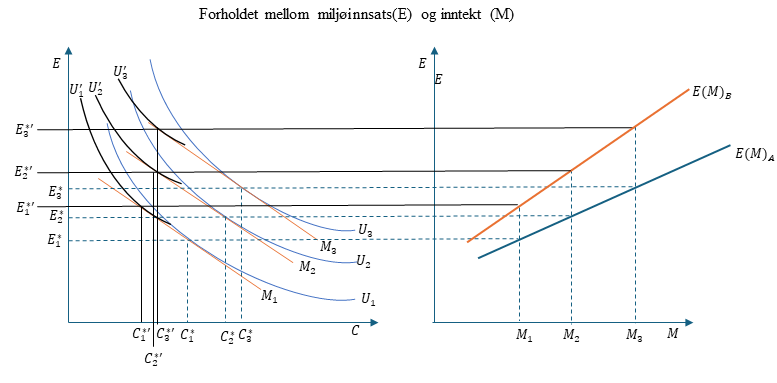
\includegraphics{Forholdet mellom E og inntekt_1.png} Figuren viser en
skisse av to situasjoner med ulike verdier av \(\alpha\) og \(\beta\) og
hvordan dette påvirker miljøinnsatsen E.

I den venstre delen av figuren har vi de to bestanddelene i
nyttefunksjonen vår C og E på henholdsvis horisontal og vertikal akse.
Budsjettlinjer for ulike nivåer av inntekt er representert ved
\(M_1\),\(M_2\) og \(M_3\) . Det er tegnet inn indifferenskurver for
nyttenivåene \(U_1\),\(U_2\) og \(U_3\) der \(\alpha\) + \(\beta\)
\textless1 og \(\alpha\) \textgreater{}\(\beta\). Disse er blå og vi
kaller dette tilfelle 1.

Tilfelle 2 i svart er vist ved \(U'_1\),\(U'_2\) og \(U'_3\) der
\(\alpha\) + \(\beta\) \textgreater1 og \(\alpha\) \textless{}
\(\beta\). Den optimale kombinasjonen av C og E vil være der
budsjettlinjen tangerer indifferenskurven. Vi ser at dette gir for
tilfelle 1 (striplete linjer) tilpasningene (\(C^*_1\), \(E^*_1\)),
(\(C^*_2\), \(E^*_2\)), (\(C^*_3\), \(E^*_3\)). Tilsvarende for tilfelle
2 blir (\(C'_1\), \(E'_1\)), (\(C'_2\), \(E'_2\)), (\(C'_3\) , \(E'_3\))
som er tegnet i helsvarte linjer. Vi ser av dette at når inntekten øker,
vil konsumet i tilfelle 1 øke mer enn miljøinnsatsen, mens i tilfelle 2
vil miljøinnsatsen øke mer enn konsumet.

I den høyre del av figuren er alle tilpasningene overført til et (M,
E)-plan som angir hvordan forløpet av E(M) vil være ved ulike verdier av
\(\alpha\) og \(\beta\). Den blå linjen er for tilfelle 1 og den
organsje for tilfelle 2. Hvis vi holder parameteren \(\alpha\) konstant
og øker parameteren \(\beta\), som begge er eksponenter i funksjonen for
forurensningsnivået \(P=C-C^\alpha E^\beta\), vil dette ha følgende
konsekvenser:

\begin{itemize}
\item
  Effekten av miljøinnsatsen \(E\) vil øke:

  Parameteret \(\beta\) bestemmer styrken av miljøinnsatsens effekt på
  forurensningsnivået. Ved å øke \(\beta\) vil en økning i
  miljøinnsatsen ha en større negativ innvirkning på
  forurensningsnivået. Dette betyr at en større økning i miljøinnsatsen
  vil føre til en proporsjonalt større reduksjon i forurensningsnivået.
\item
  Større vektlegging av miljøhensyn:

  Med økende \(\beta\) vil miljøinnsatsen få en større betydning for
  forurensningsnivået sammenlignet med konsumet. Dette kan føre til en
  sterkere oppfordring til å investere i miljøvennlige tiltak for å
  redusere forurensningen.
\item
  Mindre påvirkning fra konsumet:

  Parameteret \(\alpha\) er fortsatt konstant, så påvirkingen av
  konsumet \(C\) på forurensningsnivået forblir uendret. Imidlertid, med
  økende \(\beta\), vil den relative betydningen av konsumet i forhold
  til miljøinnsatsen reduseres, siden miljøinnsatsen får en større vekt.
  Forurensningsnivået vil falle raskere med økende miljøinnsats: Den
  økte effekten av miljøinnsatsen vil føre til en raskere reduksjon i
  forurensningsnivået når \(\beta\) øker. Dette kan ha positive
  miljømessige konsekvenser ved å oppmuntre til større investeringer i
  miljøvennlige teknologier og praksiser.
\end{itemize}

Dette innebærer at vi har identifisert preferansene til en
miljøinteressert forbruker. De vil generelt sett innebære en preferanse
for miljøvennlige produkter og tjenester, samt en preferanse for å
redusere forbruket av ressurser som bidrar til forurensning.

I appendikset viser vi hvordan forholdet mellom inntekt og forurensning
er avhengig av summen av \(\alpha\) og \(\beta\).

\hypertarget{gjennomgang-av-empirisk-forskning-puxe5-omruxe5det}{%
\subsection{2.2 Gjennomgang av empirisk forskning på
området}\label{gjennomgang-av-empirisk-forskning-puxe5-omruxe5det}}

Vi vil i det følgende presentere forskning som er gjort på dette
området. Først tar vi opp undersøkelser på BNP-nivå for deretter å vise
undersøkelser gjort med husholdsinntekt.

\textbf{Makronivå}

McConnell sier at det er tre krefter som kan bidra til formen på EKC
(McConell 1997). For det første kan det være sannsynlig at
forurensningen reduseres når inntekten øker fordi etterspørselsmønsteret
endrer seg. Med økende inntekt vil etterspørselen til husholdningene
rette seg mer mot tjenester og dermed forurense mindre. For det andre
vil handel kunne bidra gjennom større import av varer av forurensende
produksjon. På den måten vil importlandet slippe forurensingen.
Forfatterenes tredje poeng er at når inntektene øker, vil husholdningene
etterspørre mer miljøkvalitet og forvente at myndighetene gjennom lov-
og regelverk legger til rette for dette.

Resonnementet utdypes hos Andreoni (Andreoni and Levinson 2001c) som
sier i sin artikkel at det kan være flere forklaringer på den omvendte
U-formen på EKC. For det første kan dette uttrykke en naturlig økonomisk
utvikling med overgang fra et agarsamfunn til industriell produksjon og
videre til mer miljøvennlig service- og tjenesteproduksjon. Dette kan
være forårsaket av at miljøfiendlig produksjon flyttes til fattige
utviklingsland. Hvis det er dette som gir den fallende del av kurven,
vil ikke EKC kunne være forklaringsmodell for alle land fordi de
fattigste vil ikke ha noen land å eksportere sin forurensende
produksjon. En annen forklaring er at forurensning kan sees på som en
negativ eksternalitet ved produksjon. For å tvinge fram endring i
retning av reduksjon av forurensning, trengs det sterke institusjoner og
lovverk. Dette finner vi oftest og mer i industrialiserte rike land.

Roca peker på at det er to hovedretninger i forklaringene av hvorfor
forholdet mellom miljøkvalitet og inntekt framstår som en omvendt
U-kurve (Roca 2003). Den første foreslår at det er en endogen endring i
etterspørselen etter varer og tjenester. Endringen består i dreining av
etterspørselen mot varer og tjenester med lite miljøavtrykk, med
tilsvarende endring over tid i strukturen i næringslivet. Samtidig er
det viktig å analysere hva dette egentlig innebærer. Hvis et land
importerer varer som er miljøvennlig i bruk, men som er produsert på en
lite bærekraftig måte, er jo bare miljøutfordringene eksportert. Et
eksempel her er økningen i antall elektriske biler som i seg selv er
miljøvennlig tiltak, men der produksjonen av batteriene til bilene
foregår på en meget forurensende måte. Den andre retningen har også
individuelle preferanser og relativ etterspørsel etter varer og
tjenester som basis. Men her skilles det mellom etterspørsel etter
ordinære varer og tjenester og miljøkvalitet. Det antas at det er høy
inntektselastisitet i etterspørselen etter miljøkvalitet og at det er
dette som gjør at økonomisk vekst kan vedvare samtidig som presset mot
miljøet avtar.

Det er også verdt å merke seg at økende verdenshandel har medført at
miljøfiendtlig produksjon blir flyttet fra høyinntektsland med strenge
miljøreguleringer til utviklingsland med mindre vektlegging på
miljøkonsekvenser. Dette kan også være et bidrag til at forurensning er
avtakende i høyt industrialiserte land. Dette er kalt ``Polution Haven
Hypotesis'' (PHH). (Dinda 2004b), s.437.

EKC modellen har siden den gang vært anvendt på BNP per cap mot en rekke
miljøvariabler med variabelt resultat, og mange av undersøkelsene har
konkludert med at en slik sammenheng kan observeres.

Alle disse undersøkelsene tar utgangspunkt i økonomisk utvikling i land,
men det er også mange undersøkelser som ser på husholdsøkonomi og
miljøeffekter. Da endres spørsmålet til om det er en sammenheng mellom
enkeltmenneskenes økonomi og hvordan de forholder seg til
miljøutfordringer. Med andre ord, vil preferansene hos enkeltmenneskene
endre seg når inntekten endres?

\textbf{Mikronivå}

Kahn (Kahn 1998a) gjennomgikk i sin undersøkelse forholdet mellom
inntekt og utslipp av hydrokarboner fra biler på husholdningsnivå.
Bilparken i lavinntektshusholdninger vil ofte omfatte relativt gamle
biler som er dårlig vedlikeholdt med stort utslipp av klimagasser. I
husholdninger med høyere inntekter vil bilene være nyere med teknologi
som gir lavere utslipp. Det vil kanskje også være flere biler i slike
husholdninger. Resultatene viste at forholdet kan beskrives ved en
omvendt U-formet kurve, også kalt Miljø-Kuznets-kurve.

Karpinska (Karpinska and Śmiech, n.d.a) undersøkte om utslipp av
klimagasser som følge av energibruk endres med inntekten i polske
husholdninger. De fant at EKC er godt dekkende for dette forholdet. For
lave inntekter vil underforbruk av strøm og gass (fordi det er dyrt) og
mer bruk av kull og ved gi høye utslipp. Med økende inntekt vil bruken
av energikilder med lave klimagassutslipp øke, og boligene vil også være
bedre isolert.

Giovanis (Giovanis 2013a) bruker paneldata fra the Britsh Household
Survey fra 1991-2009 og ser på forholdet mellom tre mål på luftkvalitet
(Oson, Svoveldioksyd, NOX) og person- og husholdsinntekt. De bruker
flere ulike statistiske tilnærminger, men hovedkonklusjonen er at
EKC-teorien holder.

Alle disse analysene er i tråd med EKC og tilsier at med økende inntekt
vil forurensingen avta etter et visst inntektsnivå.

Til slutt vil vi trekke fram en annen innfallsvinkel fra Nauges (Nauges,
Wheeler, and Fielding 2021a). Hypotesen hans er at husholdninger i rike
land er mindre bekymret for klimaendringer fordi rikdom skaper en buffer
mot konsekvensene av endringene. Utvalget er en husholdningsundersøkelse
som omfattet 11 OECD-land og over 10 000 husholdninger. De finner et
statistisk signifikant negativt forhold mellom land- og
husholdningsrikdom og individers oppfatning av alvoret i klimaendringer.

\hypertarget{data-og-metode}{%
\section{3 Data og metode}\label{data-og-metode}}

I dette kapitlet skal vi gå gjennom data og metoden som ligger til grunn
for å gjøre vår analyse av forholdet mellom inntekt og holdninger til
miljøtiltak. Først gir vi en detaljert beskrivelse av variablene vi har
valgt i modellene, og forventet innflytelse på den avhengige variablen.
Så viser vi noe av datamaterialet som illustrasjoner. Til slutt
introduserer vi regresjonsmodellene som vi skal anvende for
undersøkelsen på hvordan ulike faktorer påvirker individets
miljøholdninger.

\hypertarget{variabler}{%
\subsection{3.1 Variabler}\label{variabler}}

Vi bruker datasett fra Norsk medborgerpanel runde 26, 2023. Denne
undersøkelsen gjennomføres årlig av Universitetet i Bergen(Ivarsflaten,
Elisabeth et al., n.d.) og undersøker holdninger og holdningsendringer i
den norske befolkningen knyttet til viktige samfunnsspørsmål. Deltakerne
blir plukket ut tilfeldig fra Folkeregistret og spurt om de vil delta på
en internettbasert undersøkelse. Datasettet består brutto av 12 021
observasjoner fordelt på 440 variabler. Vi har fått tilgang til data via
søknad. Vårt datasett består av 1 921 observasjoner når vi har valgt
variabler og tatt bort alle observasjoner som ikke hadde svart eller
ikke blitt spurt. Vi har så gjort om bakgrunnsvariablene om til
kategorier.

Den sterke reduksjonen i antall observasjoner er i første rekke knyttet
til at ikke alle respondentene er blitt spurt om alle spørsmålene i
undersøkelsen, og dette rammer våre variabler i relativt stort omfang.
Vi har sjekket hvorvidt dette går ut over representativiteten, spesielt
knyttet til inntekt, men finner ingen vesentlige forskjeller i
inntektsfordelingen i datasettet som helhet og vårt utvalg.

Vi har valgt å kalle vår avhengige variabel ``Miljøholdning''.

I undersøkelsen presenteres denne på følgende måte:

Hvor viktig mener du følgende hensyn bør være når man velger tiltak for
å redusere klimagassutslipp: Tiltaket gir utslippskutt i Norge.

Det følger også med en forklarende tekst:

\emph{En rekke tiltak er aktuelle for å redusere klimagassutslipp. Når
norske politikere skal velge mellom ulike tiltak er det flere hensyn som
må tas. Hvor viktig mener du at følgende hensyn bør være når man skal
bestemme hvilke tiltak som skal innføres?: Tiltaket gir utslippskutt i
Norge}

Det spørres altså her om hvor viktig man synes det er at tiltakene gir
utslippskutt i Norge. En høy score vil være uttrykk for høyere
miljøbevissthet enn en lav. Det vil også gi uttrykk for at man er villig
til å endre sin adferd hvis det er nødvendig. Skalaen angir hvor viktig
individet mener det er at tiltak for å redusere klimagassutslipp gir
utslippskutt i Norge. Skalaen er fra 0 til 10 hvor 0 indikerer at det
ikke er viktig i det hele tatt, mens 10 indikerer at dette er svært
viktig.

De uavhengige variablene vi har valgt er:

\textbf{Inntekt:}

Denne variabelen er vår sentrale uavhengige variabel som er basert på
vårt teoretiske grunnlag, Miljøkuznet-kurven. Den omfatter individets
bruttoinntekt og den er definert i 8 kategorier fra ``Under 150 000''
til ``mer enn 1 000 000''.

Inntekten er basert på brutto årsinntekt(inntekt før skatt) for
individet og ikke husholdningen da spørsmålet spesifikt er: ``Hva er
inntekten din for tiden? Brutto årsinntekt er:''. Vi har valgt å slå
sammen flere av kategoriene, de to laveste har vi valgt å slå sammen til
0-300 000 da denne vil dekke lavinntekstkategorien som er 60 prosent
under medianinntekten i Norge som pr 2022 er på 441 400 (Statistisk
Sentralbyrå, n.d.). For forenkling av analysen har vi slått sammen 300
til 400 tusen kategorien med 400 til 500 kategorien for å få et større
utvalg, samt 500 - 600 tusen med 600 - 700 tusen kategorien for også å
få et større utvalg samt at gjennomsnittsinntekten i Norge ligger i
dette intervallet.

Vi forventer at denne variabelen vil ha en positiv virkning på vår
avhengige variabel.

\textbf{Utdanning:}

Vi vil også se på om resultatene endrer seg hvis vi legger til en
utdanningsvariabel i regresjonen som kontrollvariabel. Vi har delt
variabelen ``høyeste fullførte utdanning'' i tre kategorier :
grunnskole, videregående skole og høyere utdanning. Vi forventer at
verdien på den avhengige variablen er økende med økt utdanningsnivå
fordi økt kunnskapsnivå har en positiv effekt på forståelse av
miljøutfordringene. Dette er i tråd med funnene til Meyer(Meyer 2015).

\textbf{Kjønn:}

Vi har tatt med kontrollvariablen kjønn for å se om det er forskjeller
mellom kvinner og menn. Vi har to kjønn i datasettet. Dette lager vi til
en dummyvariabel hvor vi setter verdien kvinne = 0 og mann = 1. Vi
ønsker å se om det er signifikante forskjeller mellom kjønnene i
holdningene, og i vår regresjon tar vi utgangpunkt i kvinnen for å se om
det er en endring/forskjell når det er en mann. I regresjonen kaller vi
denne dummyvariabelen ``kjonn''.

\textbf{Aldersgruppe:}

Denne kontrollvariabelen har vi med for å se om det er forskjell mellom
generasjonene. Aldersvariablen er delt i tre grupper: de som er født i
1959 og før, 1960-1989 og fra 1990 og etter.

\newpage

\hypertarget{deskriptiv-statistikk}{%
\subsubsection{3.1.1 Deskriptiv
statistikk}\label{deskriptiv-statistikk}}

\begin{longtable}[t]{llrrlll}
\caption{Deskriptiv statistikk}\\
\toprule
Variabel & Kategori & Antall & Prosentandel & Gjennomsnitt & Min & Max\\
\midrule
Miljøholdning & 0 & 71 & 3.70 & 6.52 & 0 & 10\\
 & 1 & 45 & 2.34 & 6.52 & 0 & 10\\
 & 2 & 76 & 3.96 & 6.52 & 0 & 10\\
 & 3 & 74 & 3.85 & 6.52 & 0 & 10\\
 & 4 & 87 & 4.53 & 6.52 & 0 & 10\\
\addlinespace
 & 5 & 274 & 14.26 & 6.52 & 0 & 10\\
 & 6 & 211 & 10.98 & 6.52 & 0 & 10\\
 & 7 & 282 & 14.68 & 6.52 & 0 & 10\\
 & 8 & 333 & 17.33 & 6.52 & 0 & 10\\
 & 9 & 203 & 10.57 & 6.52 & 0 & 10\\
\addlinespace
 & 10 & 265 & 13.79 & 6.52 & 0 & 10\\
Inntekter & 0 - 300 000 & 211 & 10.98 &  &  & \\
 & 300 001 - 500 000 & 589 & 30.66 &  &  & \\
 & 500 001 - 700 000 & 560 & 29.15 &  &  & \\
 & 700 001 - 1 000 000 & 358 & 18.64 &  &  & \\
\addlinespace
 & Mer enn 1 000 000 & 203 & 10.57 &  &  & \\
Utdanning & grunnskole & 79 & 4.11 &  &  & \\
 & videregående & 613 & 31.91 &  &  & \\
 & høyere & 1229 & 63.98 &  &  & \\
Kjønn & Mann & 1026 & 53.41 &  &  & \\
\addlinespace
 & Kvinne & 895 & 46.59 &  &  & \\
Aldersgruppe & 1959\_og\_før & 837 & 43.57 &  &  & \\
 & 1960\_1989 & 952 & 49.56 &  &  & \\
 & 1990\_og\_etter & 132 & 6.87 &  &  & \\
\bottomrule
\end{longtable}

I tabell 1 Deskriptiv statistikk finner vi oversikt over alle variablene
og fakta om dem. Utvalget vårt er totalt 1921 observasjoner.

\hypertarget{noen-grafiske-illustrasjoner}{%
\subsection{3.2 Noen grafiske
illustrasjoner}\label{noen-grafiske-illustrasjoner}}

Vi vil her visualisere noe av det vi har funnet i datasettet. Dette kan
gi nyttige bakgrunnsinformasjon for forståelse av analyse og resultater.

\hypertarget{inntektsfordeling-mellom-kjuxf8nn}{%
\subsubsection{\texorpdfstring{\textbf{3.2.1 Inntektsfordeling mellom
kjønn}}{3.2.1 Inntektsfordeling mellom kjønn}}\label{inntektsfordeling-mellom-kjuxf8nn}}

Det første vi ser på er inntektsfordelingen mellom kjønnene.

\begin{figure}[H]

{\centering \includegraphics{Bacheloroppgave_kandidat_12_og_39_files/figure-pdf/fig-inntekt-1.pdf}

}

\caption{\label{fig-inntekt}Inntekt fordelt på inntektsgruppene i
prosent}

\end{figure}

Av Figur~\ref{fig-inntekt} ser vi at kvinner er overrepresentert i den
laveste inntektsgruppen, men menn er overrepresentert i de to høyeste.
For inntekter mellom 300 000 - 700 000 er det lik fordeling mellom
kjønnene.

\hypertarget{forholdet-mellom-kjuxf8nn-og-utdanning}{%
\subsubsection{3.2.2 Forholdet mellom kjønn og
utdanning}\label{forholdet-mellom-kjuxf8nn-og-utdanning}}

Vi har også sett på hvordan utdanningsnivået er fordelt mellom kjønnene.

\begin{figure}[H]

{\centering \includegraphics{Bacheloroppgave_kandidat_12_og_39_files/figure-pdf/fig-utdanning-1.pdf}

}

\caption{\label{fig-utdanning}Utdanning fordelt på kjønn i prosent}

\end{figure}

Vi ser av Figur~\ref{fig-utdanning} at det er store forskjeller mellom
kjønnene på de laveste utdanningsnivåene, men for høyere utdanning er et
relativt lik fordeling.

\hypertarget{regresjonsmodellene}{%
\subsection{3.3 Regresjonsmodellene}\label{regresjonsmodellene}}

Vi bruker multippel regresjonanalyse fordi vi i utgangspunktet vurderer
det slik at det er flere variabler som påvirker vår avhengige variabel,
og vi ønsker å finne ut om det er en statistisk sammenheng mellom våre
uavhengige variabler og vår avhengige variabel. Vi vil bruke minste
kvadraters metode fordi den finner de verdiene av
regresjonskoeffisientene som gir oss den minste kvadratsummen av
residualene og dermed regresjonsflaten som i gjennomsnitt er nærmest
alle de observerte individuelle datapunktene (Mehmetoglu and Mittner
2020).

Minste kvadraters metode bygger på noen forutsetninger som vi vil teste
etter hvert. Disse er:

\begin{enumerate}
\def\labelenumi{\arabic{enumi}.}
\item
  Det må være en lineær sammenheng mellom variabler slik at den
  avhengige variabelen kan uttrykkes som en lineær funksjon av de
  uavhengige variablene.
\item
  Residualene(feiltermene) antas å være normalfordelt. Dette betyr at
  feilene rundt den lineære tilpasningen bør følge en normalfordeling,
  noe som gjør det mulig å bruke statistiske metoder for å evaluere
  modellen.
\item
  Variansen til feiltermene er konstant over hele spennet av de
  uavhengige variablene. Dette kalles homoskedastisitet og betyr at
  spredningen av feilene antas å være konstant langs x-aksen.
\item
  Det antas at det ikke er noen lineær avhengighet mellom de uavhengige
  variablene. Dette innebærer ingen perfekt multikollinearitet.
\end{enumerate}

Vi vil ta utgangspunkt i et signifikansnivå på 5 \%.

Vi vil bruke totalt seks regresjonsmodeller basert på de nevnte
uavhengige variablene

Modell 1: \(Miljoholdning=\beta_0 + \beta_1inntekter + \epsilon_i\ \)

Modell 2:
\(Miljoholdning=\beta_0 + \beta_1inntekter + \beta_2utdanning + \epsilon_i\ \)

Modell 2 undersøker om det er noen interaksjonseffekter mellom inntekter
og utdanning. Dette vil si at vi ser etter om effekten som inntekt har
på miljøholdning er avhengig av nivået på utdanning.

Modell 2a:
\(Miljoholdning=\beta_0 + \beta_1inntekter + \beta_2utdanning + \beta_1inntekter *\beta_2utdanning + \epsilon_i\ \)

Modell 3:
\(Miljoholdning=\beta_0 + \beta_1inntekter + \beta_2utdanning + \beta_3Kjonn + \epsilon_i\ \)

Modell 3a undersøker om det er noen interaksjonseffekter mellom
utdanning og kjønn. Dette vil si at vi ser etter om effekten som
utdanning har på miljøholdning er avhengig av kjønn.

Modell 3a:
\(Miljoholdning=\beta_0 + \beta_1inntekter + \beta_2utdanning + \beta_3Kjonn + \beta_2utdanning*\beta_3Kjonn + \epsilon_i\ \)

Modell 4:
\(Miljoholdning=\beta_0 + \beta_1inntekter + \beta_2utdanning + \beta_3Kjonn + \beta_4Aldersgruppe + \epsilon_i\ \)

Konstantleddet \(\beta_0\) angir verdien på den avhengige variablen når
alle uavhengige er lik 0. Regresjonskoeffisienten \(\beta_i\) angir den
gjennomsnittlige effekten de uavhengige variabelene har på den avhengige
variabelen tiltak\_utslippskutt når vi holder verdien på de andre
variablene konstant. \(\epsilon_i\) er et restledd for all annen
påvirkning.

\hypertarget{resultater}{%
\section{4 Resultater}\label{resultater}}

Vi vil her vise den empiriske analysen og resultatene vi har kommet fram
til. Vi vil gjennomgå en regresjonsmodell med flere variabler. Det er
også gjennomfør ulike tester for å vurdere den mest omfattende modellen.
Vår null-hypotese til modellen er at det ikke er noen sammenheng mellom
inntekt og holdning til tiltak som gir utslippskutt i Norge. Den
alternative hypotesen blir at det er en sammenheng. Signifikansnivået er
satt til 5 \%. Dette betyr at hvis vi finner p-verdier lavere enn 0,05,
skal null-hypotesen avvises til fordel for den alternative hypotesen.

Vi vil også gjennomføre analyser der vi legger til utdanningsnivå, kjønn
og aldersgruppe som kontrollvariabler for å se om dette vil ha
innflytelse på vår avhengige variabel.

\hypertarget{regresjonsmodeller}{%
\subsection{4.1 Regresjonsmodeller}\label{regresjonsmodeller}}

Den avhengige variabelen er hvor viktig individet mener det er at tiltak
for å redusere klimagassutslipp gir utslippskutt i Norge. Den har vi
kalt ``Miljøholdning''.

\hypertarget{oversikt-over-resultatene}{%
\subsubsection{4.2.1 Oversikt over
resultatene}\label{oversikt-over-resultatene}}

For lesbarhetens skyld har vi delt resultatene på to tabeller. Den
første viser resultatene for modell 1, modell 2 og modell 2a, mens den
siste viser modell 3, modell 3a og modell 4.

\begin{verbatim}

==============================================================================================================
                                                    modell_1            modell_2            modell_2a         
--------------------------------------------------------------------------------------------------------------
(Intercept)                                            6.66 (0.18) ***     6.37 (0.32) ***     5.92 (0.52) ***
inntekter300 001 - 500 000                             0.12 (0.21)         0.00 (0.21)         0.66 (0.67)    
inntekter500 001 - 700 000                            -0.07 (0.21)        -0.33 (0.22)         0.68 (0.98)    
inntekter700 001 - 1 000 000                          -0.52 (0.23) *      -0.80 (0.23) ***    -0.25 (1.59)    
inntekterMer enn 1 000 000                            -0.58 (0.26) *      -0.90 (0.26) ***    -1.25 (1.59)    
utdanningvideregående                                                      0.08 (0.31)         0.78 (0.58)    
utdanninghøyere                                                            0.72 (0.31) *       0.93 (0.61)    
inntekter300 001 - 500 000:utdanningvideregående                                              -0.88 (0.73)    
inntekter500 001 - 700 000:utdanningvideregående                                              -1.71 (1.03)    
inntekter700 001 - 1 000 000:utdanningvideregående                                            -0.52 (1.64)    
inntekterMer enn 1 000 000:utdanningvideregående                                               0.28 (1.68)    
inntekter300 001 - 500 000:utdanninghøyere                                                    -0.46 (0.75)    
inntekter500 001 - 700 000:utdanninghøyere                                                    -0.63 (1.03)    
inntekter700 001 - 1 000 000:utdanninghøyere                                                  -0.39 (1.63)    
inntekterMer enn 1 000 000:utdanninghøyere                                                     0.57 (1.64)    
--------------------------------------------------------------------------------------------------------------
R^2                                                    0.01                0.02                0.03           
Adj. R^2                                               0.01                0.02                0.02           
Num. obs.                                           1921                1921                1921              
==============================================================================================================
*** p < 0.001; ** p < 0.01; * p < 0.05
\end{verbatim}

\newpage

\begin{verbatim}

========================================================================================
                              modell_3            modell_3a           modell_4          
----------------------------------------------------------------------------------------
(Intercept)                      6.86 (0.32) ***     7.18 (0.50) ***     6.87 (0.33) ***
inntekter300 001 - 500 000       0.21 (0.21)         0.25 (0.21)         0.32 (0.21)    
inntekter500 001 - 700 000      -0.08 (0.22)        -0.03 (0.22)         0.12 (0.22)    
inntekter700 001 - 1 000 000    -0.37 (0.24)        -0.34 (0.24)        -0.09 (0.25)    
inntekterMer enn 1 000 000      -0.36 (0.27)        -0.34 (0.27)        -0.05 (0.28)    
utdanningvideregående           -0.03 (0.31)        -0.26 (0.52)         0.01 (0.31)    
utdanninghøyere                  0.41 (0.31)         0.00 (0.51)         0.40 (0.31)    
Kjonn                           -1.01 (0.12) ***    -1.53 (0.61) *      -1.06 (0.13) ***
utdanningvideregående:Kjonn                          0.32 (0.65)                        
utdanninghøyere:Kjonn                                0.64 (0.63)                        
Aldersgruppe1960_1989                                                   -0.37 (0.13) ** 
Aldersgruppe1990_og_etter                                                0.39 (0.25)    
----------------------------------------------------------------------------------------
R^2                              0.06                0.06                0.06           
Adj. R^2                         0.05                0.05                0.06           
Num. obs.                     1921                1921                1921              
========================================================================================
*** p < 0.001; ** p < 0.01; * p < 0.05
\end{verbatim}

\hypertarget{modell-1-med-inntekt}{%
\subsubsection{4.1.2 Modell 1 med inntekt}\label{modell-1-med-inntekt}}

Hovedmodellen vår er å se på om det er noen sammenheng mellom inntekt og
vår uavhengige variabel.

\textbf{Tolkning av resultatet:}

Intercepten representerer konstantleddet i modellen og forteller oss at
forventet verdi på holdningsskalaen vil være 6,66 når inntekten er i
intervallet 0 - 300 000. Estimatene for inntektsgruppene 700 000 - 1 000
000 og Mer enn 1 000 000 faller med henholdsvis 0,52 og 0,58. Verdiene
er signifikante og innebærer at vi kan med 95 \% sikkerhet si at det er
en negativ sammenheng mellom inntekt på disse nivåene og miljøholdning.

Adjusted \(R^2\) gir oss at variablene i regresjonslikningen i denne
modellen forklarer kun 1 prosent av sammenhengen. Dette betyr at det er
mange andre forhold som er med på å forklare sammenhengen, men som ikke
er med i analysen.

\hypertarget{modell-2-med-inntekt-og-utdanning}{%
\subsubsection{4.1.3 Modell 2 med inntekt og
utdanning}\label{modell-2-med-inntekt-og-utdanning}}

I denne modellen har vi utvidet vår modell med en utdanningsvariabel på
tre nivå, grunnskole, videregående og høyere utdanning.

\textbf{Tolkning av modellen:}

Intercepten er konstantleddet i regresjonsmodellen vår og sier at den
forventede verdien på holdningsskalaen er 6.37 når inntekten er under
300 000 og utdanningsnivået er grunnskole. For inntekter over 700 000
til 1 mill reduseres den forventede verdien på holdningsskalaen med 0,8
poeng til 5,57. P-verdien er 0 og dermed er denne sammenhengen
signifikant. Dette innebærer at det er en negativ sammenheng mellom
inntekt og miljøholdning med grunnskoleutdanning for denne
inntektsgruppen. Hvis inntekten er over 1 mill reduseres verdien med 0.9
til 5,47 . Dette resultatet er også signifikant og angir en negativ
sammenheng. Vi finner altså at med lavt utdanningsnivå er
miljøholdningen fallende når inntekten er over 700 000. Hvis
utdanningsnivået er høyere utdanning, vil estimatet øke med 0,72 for
hver av inntektsgruppene. Dette resultatet er signifikant, men selv med
høy utdanning i de høyeste inntektsgruppene er estimatet fortsatt
negativt, men i mye mindre grad. Vårt funn er derfor at høy utdanning
kan ha en dempende virkning på effekten av økende inntekt.

Oppsummert gir dette oss at vi finner en negativ sammenheng mellom
inntekt og miljøholdninger for inntekter over 700 000 når vi
kontrollerer for effekten av utdanning. Utdanning ser ut til å ha en
dempende virkning på den negative sammenhengen.

Adjusted \(R^2\) forteller oss at variablene i regresjonslikningen i
modell 2 forklarer 2 prosent av sammenhengen. Dette betyr at det
fremdeles er mange andre forhold som er med på å forklare sammenhengen,
men som ikke er med i analysen.

\hypertarget{modell-2a-med-inntekt-utdanning-og-interaksjon-mellom-inntekt-og-utdanning}{%
\subsubsection{4.1.4 Modell 2a med inntekt, utdanning og interaksjon
mellom inntekt og
utdanning}\label{modell-2a-med-inntekt-utdanning-og-interaksjon-mellom-inntekt-og-utdanning}}

Her tester vi om effekten som inntekt har på miljøholdning er avhengig
av nivået på utdanning. Av resultatene for denne modellen ser vi at
konstantleddet(intercepten) gir oss en forventet verdi på
holdningsskalaen på 5,92 når inntekten er under 300 000 og
utdanningsnivået er grunnskole. Denne er signifikant. Det er ingen andre
signifikante resultater i denne modellen og finner heller ingen
sigifikant interaksjonseffekt.

\hypertarget{modell-3-med-inntekt-utdanning-og-kjuxf8nn}{%
\subsubsection{4.1.5 Modell 3 med inntekt, utdanning og
kjønn}\label{modell-3-med-inntekt-utdanning-og-kjuxf8nn}}

Vi utvider modellen til også å omfatte kjønn for å se på om det er
forskjeller mellom kvinner og menn.

\textbf{Tolkning av resultatene}

Av resultatene for denne regresjonsmodellen modellen ser vi at
konstantleddet(intercepten) gir oss en forventet verdi på
holdningsskalaen på 6.86 for kvinner når inntekten er under 300 000 og
utdanningsnivået er grunnskole. Denne er signifikant For menn reduseres
estimatet med 1,01 på holdningsskalaen. Dette resultatet er signifikant.

Vi ser at adjusted \(R^2\) nå har økt til 5 \%. Dette betyr at den nye
variabelen i regresjonslikningen i modell 3 har forklaringskraft, men
det er fremdeles mange andre forhold som er med på å forklare
sammenhengen, men som ikke er med i analysen.

\hypertarget{modell-3a-med-inntekt-utdanning-og-kjuxf8nn-og-interaksjon-utdanning-kjuxf8nn}{%
\subsubsection{4.1.6 Modell 3a med inntekt, utdanning og kjønn og
interaksjon
utdanning-kjønn}\label{modell-3a-med-inntekt-utdanning-og-kjuxf8nn-og-interaksjon-utdanning-kjuxf8nn}}

\textbf{Tolkning av modellen:}

Modell 3a omfatter modell 3 og en interaksjonsvariabel mellom kjønn og
utdanning. Vi ser om effekten som utdanning har på miljøholdning er
avhengig av kjønn. Av resultatene for denne regresjonsmodellen modellen
ser vi at konstantleddet(intercepten) gir oss en forventet verdi på
holdningsskalaen på 7,18 for kvinner når inntekten er under 300 000 og
utdanningsnivået er grunnskole. Denne er signifikant. For menn reduseres
estimatet med 1,53 på holdningsskalaen. Dette resultatet er også
signifikant. Vi finner ingen sigifikant interaksjonseffekt.

\hypertarget{modell-4-med-inntekt-utdanning-og-kjuxf8nn-og-aldersgruppe}{%
\subsubsection{4.1.7 Modell 4 med inntekt, utdanning og kjønn og
aldersgruppe}\label{modell-4-med-inntekt-utdanning-og-kjuxf8nn-og-aldersgruppe}}

\textbf{Tolkning av modellen:}

For modell 4 har vi signifikant estimat for miljøholdning på 6,87 på
konstantleddet(intercepten). Dette omfatter kvinner med inntekten under
300 000 og grunnskole som utdanningsnivå og født før 1960.
Kjønnsvariablen viser at også her er resultatet for menn vesenlig lavere
og signifikant. Vi ser aldersgruppen1960-1989 trekker ned
holdningsestimatet. Dette resultatet er signifikant.

\newpage

\hypertarget{diskusjon-og-konklusjon}{%
\section{5 Diskusjon og konklusjon}\label{diskusjon-og-konklusjon}}

Vår problemstilling er om det er en sammenheng mellom inntekt og
holdninger til klimagasstiltak som gir utslippskutt i Norge.

I våre modeller er den avhengige variablen hvor viktig individet mener
det er at tiltak for å redusere klimagassutslipp gir utslippskutt i
Norge. Vi har kaldt den miljøholdning. Våre resultater for modell 1
antyder at for høye inntekter blir scoren for miljøholdning avtakende.
Dette innebærer at de positive miljøholdningene blir svakere når
inntekten er høy. Når vi i modell 2 utvider med en utdanning som
kontrollvariabel, ser vi at høyere utdanning vil kompensere noe for
dette, men at scoren likevel vil gå ned. Vår modell 2a har med
interaksjon mellom inntekt og utdanning i tillegg. Av resultatene ser vi
at effekten som inntekt har på miljøholdning ikke er avhengig av nivået
på utdanning. I vår tredje modell der kjønn er tatt med, ser vi at det
er signifikante forskjeller mellom kjønnene, men ikke på inntekt og
utdanning. Dette kan ha sammenheng med at det er stor forskjell i
inntektsfordelingen mellom menn og kvinner i de høyeste
inntektsgruppene. 3a omfatter modell 3 og en interaksjonsvariabel mellom
kjønn og utdanning. Vi finner at effekten som utdanning har på
miljøholdning ikke er avhengig av kjønn. Modell 4 omfatter også
aldersgruppe. Vi finner her at kjønn og aldersgruppe 1960\_1989 har
signifikant betydning for miljøholdning.

Vi ser at når regresjonen utvides med flere kontrollvariabler,
forsvinner de signifikante resultatene vi fant for inntekter over 700
000. Dette kan bety at kjønn har større betydning enn inntekt for
miljøholdning. Det kan også innebære at kjønn og aldersgruppe har større
betydning enn inntekt for miljøholdning.

Teorien om EKC sier at når inntekten når et visst punkt, vil
forurensningen avta fordi miljøinnsatsen øker(Kahn 1998b),(Karpinska and
Śmiech, n.d.b), (Giovanis 2013b). Dette kan for eksempel skyldes at
konsumentene endrer forbruksmønster når inntekten øker. Vi finner ikke
dette i våre resultater fordi den positive miljøholdningen avtar når
inntekten går over 700 000.

Hos Nauges(Nauges, Wheeler, and Fielding 2021b) gir empiriske funn grunn
til å vurdere om det kan være slik at miljøinnsatsen faller etter et
visst inntektsnivå fordi det kan være en oppfatning at man kan kjøpe seg
ut av konsekvensene av klimaendringene. For veldig høye inntekter kan
dette gi lavere miljøscore. Det kan også være at interessen for
miljøutfordringene i Norge er dalende for de rikeste fordi de ikke er så
opptatt av eget lands bidrag.

Slik vi vurderer det, er våre funn i modell 1 i tråd med Nauges fordi
regresjonen bare omfatter forholdet mellom miljøholdninger(her:
miljøinnsatsen) og inntekt. Når det gjelder modell 2 vil man kunne anta
at utdanning som en kunnskapsleverandør vil kunne gi bidrag til økt
miljøforståelse og dermed ha positiv virkning på miljøholdningene.

For vår undersøkelse ser vi noen begrensninger i bruk av EKC- modellen.
For det første er de fleste forskningsresultatene gjort på makronivå med
BNP og land som variabler. Det er også gjort noen undersøkelser med
husholdsinntekt som uavhengig variabel, men den avhengige variabelen er
ofte i konkret form som for eksempel direkte reduksjon av \(CO_2\). Vi
er ikke kjent med undersøkelser der den avhengige variabelen er antatt å
være et uttrykk for forurensning. For det andre er det store variasjoner
i resultatene fra de empiriske undersøkelsene, og det er en pågående
diskusjon om hvorvidt vi kan snakke om en stabil sammenheng mellom
inntekt og forurensning.\\
Datasettet besto brutto av 12 021 observasjoner. Vårt datasett ble til
slutt 1 921 observasjoner fordi vi har tatt bort alle observasjoner som
ikke hadde svart eller ikke blitt spurt. Utvalget ble derfor relativt
lite. Dette kan føre til at det blir skjevheter i variablene. Noen
ekstremverdier kan dermed gi store utslag. Det kan også oppstå
skjevheter som en følge av at respondentene ikke har ønsket å svare på
grunn av lav interesse for problemstillingen.

For inntektsvariablen ser vi at for hele datasettet vårt er det
noenlunde samme inntektsfordeling som i det store datasettet samlet
sett, men det er en stor forskjell mellom kvinner og menn i de to
høyeste inntektsgruppene. Dette vil påvirke resultatene våre i modell 3.
Vi viser her til Figur~\ref{fig-inntekt} som beskriver dette.
Inntektsvariabelen er ikke kontinuerlig, noe som begrenser analysen. Den
burde også være relatert til fulltidsarbeid.

Vi ser at det er tildels store forskjeller i utdanningsnivå i det store
datasettet og vårt. Dette gjelder både mellom kjønn og totalt. Dette kan
også ha påvirket resultatene.

Det kan stilles spørsmål ved om vi faktisk har målt det vi ønsker å
måle. Vi ønsket å undersøke om det er en sammenheng mellom inntekt og
holdningene til tiltak som reduserer klimagassutslipp, og har teoretisk
brukt variabelen miljøinnsats. Koblingen er at holdningene kommer til
syne i miljøinnsats ved endring i personlig adferd og forbruksmønster
som i sin tur påvirker klimagassutslipp og dermed forurensning.

\hypertarget{konklusjon}{%
\paragraph{Konklusjon}\label{konklusjon}}

\begin{itemize}
\item
  Det kan være begrensende at det er inntektsnivået som er en viktig
  kilde til miljøinnsats . Ulike miljøtiltak med formål om
  utslippsreduksjon må favne videre slik at alle i samfunnet ser
  viktigheten av dette uavhengig av inntekt og utdanning.
\item
  Vi ser at utdanning har stor betydning i vår regresjon. Utdanning
  betyr kunnskap om hvordan det hele henger sammen. Dette kan bety at
  tiltak som legger vekt å gi ny kunnskap er en viktig kilde til å øke
  miljøfokus.
\item
  Det kan derfor se ut som at det viktigste vil være å utforme tiltak
  som appellerer til at det er en felles framtid uavhengig av inntekt og
  kjønn osv og at hvis det skal være en framtid må alle bidra.
\end{itemize}

\newpage

\hypertarget{appendiks}{%
\section{Appendiks}\label{appendiks}}

\hypertarget{test-av-forutsetningene-for-metoden}{%
\subsection{1 Test av forutsetningene for
metoden}\label{test-av-forutsetningene-for-metoden}}

Vi vil her gå gjennom noen tester for å se om forutsetningene for å
bruke OLS er oppfylt og viser her til 3.2 der disse gjennomgås. Testene
er bare utført for den enkleste modellen(modell1). Mer

\hypertarget{lineuxe6r-sammenheng-mellom-variablene}{%
\subsubsection{2.1 Lineær sammenheng mellom
variablene}\label{lineuxe6r-sammenheng-mellom-variablene}}

Denne testen tar for seg forutsetningen om lineær sammenheng og dette
plottet tar viser hvorvidt residualene har ikke-lineære mønstre.

\begin{figure}[H]

{\centering \includegraphics{Bacheloroppgave_kandidat_12_og_39_files/figure-pdf/unnamed-chunk-17-1.pdf}

}

\end{figure}

Vi ser at verdiene er jevnt fordelt rundt den horisontale linjen og kan
konkludere med at forutsetningen er oppfylt.

\hypertarget{normalfordelte-residualerfeiltermer}{%
\subsubsection{1.2 Normalfordelte
residualer(feiltermer)}\label{normalfordelte-residualerfeiltermer}}

Vi sjekker her om residualene er normalfordelt. Hvis dette er tilfelle,
vil de følge en rett linje uten store avvik.

\begin{figure}[H]

{\centering \includegraphics{Bacheloroppgave_kandidat_12_og_39_files/figure-pdf/unnamed-chunk-18-1.pdf}

}

\end{figure}

Vi ser av figuren at residualene ligger under den ideelle linjen for
lave og høye verdier. Konklusjon er at residualene er ganske
normalfordelte.

\hypertarget{konstant-varians-hos-feiltermenehomoskedastisitet.}{%
\subsubsection{1.3 Konstant varians hos
feiltermene(homoskedastisitet).}\label{konstant-varians-hos-feiltermenehomoskedastisitet.}}

Dette plottet viser om variansen til residualene er konstant.

\begin{figure}[H]

{\centering \includegraphics{Bacheloroppgave_kandidat_12_og_39_files/figure-pdf/unnamed-chunk-19-1.pdf}

}

\end{figure}

Vi ser at spredningen er noenlunde jevn rundt linjen og kan konkludere
med at variansen hos feiltermene er noenlunde konstant.

\hypertarget{kolinearitet}{%
\subsubsection{1.4 Kolinearitet}\label{kolinearitet}}

Denne testen sjekker om det er noen lineær sammenheng mellom to
variabler.

\begin{verbatim}
                 GVIF Df GVIF^(1/(2*Df))
inntekter    1.518449  4        1.053598
utdanning    1.193774  2        1.045275
Kjonn        1.150469  1        1.072599
Aldersgruppe 1.286356  2        1.064977
\end{verbatim}

Vi ser at VI-verdiene er i nærheten av 1 alle sammen noe som indikerer
at det ikke er noen lineært forhold mellom variablene.

\hypertarget{ekstremverdier}{%
\subsubsection{2.5 Ekstremverdier}\label{ekstremverdier}}

Dette plottet viser om noen av verdiene er ekstremverdier som kan
påvirke regresjonen

\begin{figure}[H]

{\centering \includegraphics{Bacheloroppgave_kandidat_12_og_39_files/figure-pdf/unnamed-chunk-21-1.pdf}

}

\end{figure}

Vi ser at vi har noen utliggere på inntekt som kan påvirke resultatene.

Samlet vil vi konkludere med at testene viser at forutsetningene for OLS
er oppfylt.

\hypertarget{mer-om-environmental-kuznets-curveekc}{%
\subsection{2 Mer om Environmental Kuznets
Curve(EKC)}\label{mer-om-environmental-kuznets-curveekc}}

Her viser vi hvordan forholdet mellom inntekt og forurensning er
avhengig av summen av \(\alpha\) og \(\beta\).

Den deriverte av likning~\ref{eq-sol_P} angir stigningstallet til
\(P(M)\):
\begin{equation}\protect\hypertarget{eq-sol_P_1-derivert}{}{ \frac{\partial P^*}{\partial M} = \frac{\alpha}{\alpha+\beta} -(\alpha+\beta) (\frac{\alpha}{\alpha+\beta})^\alpha (\frac{\beta}{\alpha+\beta})^\beta M^{\alpha+\beta-1}}\label{eq-sol_P_1-derivert}\end{equation}

Det er verdien på summen av \(\alpha\) og \(\beta\) som avgjør hvorvidt
kurven er stigende eller fallende. La oss se nærmere på dette:

\begin{itemize}
\item
  Hvis \(\alpha+\beta = 1\) vil tiltak mot forurensning ha konstant
  skalavirkning og \(\frac{\partial P^*}{\partial M}\) vil være
  konstant.
\item
  Hvis \(0 \leq \alpha\) og \(\beta \leq 1\) vil forurensingsnivået
  \(P^*\) øke proposjonalt med M.
\item
  Hvis \(\alpha+\beta \neq1\) kan vi se nærmere på den andrederiverte
  til likning~\ref{eq-sol_P_1-derivert} for å finne ut om vi har et
  toppunkt eller bunnpunkt:
  \begin{equation}\protect\hypertarget{eq-sol_P_2-derivert}{}{ \frac{\partial^2 P^*}{\partial M^2} =-(\alpha+\beta-1)(\alpha+\beta) (\frac{\alpha}{\alpha+\beta})^\alpha (\frac{\beta}{\alpha+\beta})^\beta M^{\alpha+\beta-2}}\label{eq-sol_P_2-derivert}\end{equation}
\end{itemize}

Hvis fortegnet til den andrederiverte er positivt, vil kurven være
konveks og negativt vil gi konkav kurve.

\begin{itemize}
\item
  Hvis \(\alpha+\beta < 1\) vil dette gi positivt fortegn og tiltak mot
  forurensning ha avtakende skalavirkning. \(P^*(M)\) vil være konveks.
\item
  Hvis \(\alpha+\beta > 1\) vil dette gi positivt fortegn og tiltak mot
  forurensning ha økende skalavirkning. \(P^*(M)\) vil være konkav. Det
  er denne kurven som blir omtalt som miljø-Kuznets kurven(EKC).
\end{itemize}

Figuren viser en illustrasjon av de tre tilfellene. Tilfelle (iii) er
EKC.

\begin{figure}[H]

{\centering \includegraphics{Bacheloroppgave_kandidat_12_og_39_files/figure-pdf/fig-kuznet-1.pdf}

}

\caption{\label{fig-kuznet}Kurveforløp for ulike verdier av alfa og
beta}

\end{figure}

\hypertarget{variabelliste}{%
\subsection{3 Variabelliste}\label{variabelliste}}

Dette er en oversikt over de variablene vi har brukt i modellene og kode
de har i det opprinnelige datasettet:

\begin{itemize}
\item
  Miljøholdning = r26k2\_cemes\_e
\item
  Inntekt = r26k2\_bginc
\item
  Utdanning = r26P4\_1
\item
  Kjønn =r26P1
\item
  Fødselsår = r26P5\_2
\end{itemize}

\hypertarget{referanser}{%
\section*{7 Referanser}\label{referanser}}
\addcontentsline{toc}{section}{7 Referanser}

\hypertarget{refs}{}
\begin{CSLReferences}{1}{0}
\leavevmode\vadjust pre{\hypertarget{ref-andreoni2001}{}}%
Andreoni, James, and Arik Levinson. 2001a. {``The Simple Analytics of
the Environmental Kuznets Curve.''} \emph{Journal of Public Economics}
80 (2): 269--86. \url{https://doi.org/10.1016/S0047-2727(00)00110-9}.

\leavevmode\vadjust pre{\hypertarget{ref-andreoni2001a}{}}%
---------. 2001b. {``The Simple Analytics of the Environmental Kuznets
Curve.''} \emph{Journal of Public Economics} 80 (2): 269--86.
\url{https://doi.org/10.1016/S0047-2727(00)00110-9}.

\leavevmode\vadjust pre{\hypertarget{ref-andreoni2001b}{}}%
---------. 2001c. {``The Simple Analytics of the Environmental Kuznets
Curve.''} \emph{Journal of Public Economics} 80 (2): 269--86.
\url{https://doi.org/10.1016/S0047-2727(00)00110-9}.

\leavevmode\vadjust pre{\hypertarget{ref-dinda2004}{}}%
Dinda, Soumyananda. 2004a. {``Environmental Kuznets Curve Hypothesis: A
Survey.''} \emph{Ecological Economics} 49 (4): 431--55.
\url{https://doi.org/10.1016/j.ecolecon.2004.02.011}.

\leavevmode\vadjust pre{\hypertarget{ref-dinda2004a}{}}%
---------. 2004b. {``Environmental Kuznets Curve Hypothesis: A
Survey.''} \emph{Ecological Economics} 49 (4): 431--55.
\url{https://doi.org/10.1016/j.ecolecon.2004.02.011}.

\leavevmode\vadjust pre{\hypertarget{ref-giovanis2013}{}}%
Giovanis, Eleftherios. 2013a. {``Environmental Kuznets Curve: Evidence
from the British Household Panel Survey.''} \emph{Economic Modelling} 30
(January): 602--11. \url{https://doi.org/10.1016/j.econmod.2012.10.013}.

\leavevmode\vadjust pre{\hypertarget{ref-giovanis2013a}{}}%
---------. 2013b. {``Environmental Kuznets Curve: Evidence from the
British Household Panel Survey.''} \emph{Economic Modelling} 30
(January): 602--11. \url{https://doi.org/10.1016/j.econmod.2012.10.013}.

\leavevmode\vadjust pre{\hypertarget{ref-grossman1991}{}}%
Grossman, Gene, and Alan Krueger. 1991. {``Environmental Impacts of a
North American Free Trade Agreement.''} Cambridge, MA.
\url{https://doi.org/10.3386/w3914}.

\leavevmode\vadjust pre{\hypertarget{ref-ivarsflatenelisabethetal.a}{}}%
Ivarsflaten, Elisabeth et al. n.d. {``Norsk medborgerpanel runde 26
2023.''}
\url{https://surveybanken.sikt.no/no/study/547be65b-fb02-480a-9192-6781233cdd17/undefined?type=studyMetadata\&elements=\%5B\%2272771119-0ced-422c-bc97-01b89cb4e658/4\%22\%5D\&datafile=5343ae2b-5f89-42d2-83c0-ec1bf7a97651/10}.

\leavevmode\vadjust pre{\hypertarget{ref-kahn1998}{}}%
Kahn, Matthew E. 1998a. {``A Household Level Environmental Kuznets
Curve.''} \emph{Economics Letters} 59 (2): 269--73.
\url{https://doi.org/10.1016/S0165-1765(98)00035-4}.

\leavevmode\vadjust pre{\hypertarget{ref-kahn1998a}{}}%
---------. 1998b. {``A Household Level Environmental Kuznets Curve.''}
\emph{Economics Letters} 59 (2): 269--73.
\url{https://doi.org/10.1016/S0165-1765(98)00035-4}.

\leavevmode\vadjust pre{\hypertarget{ref-karpinska2022a}{}}%
Karpinska, Lilia, and Sławomir Śmiech. n.d.a. {``Environmental Kuznets
Curve At Home? New Evidence On CO2 Emissions and Income of Polish
Households Living In Detached Houses.''}
\url{https://doi.org/10.2139/ssrn.4151899}.

\leavevmode\vadjust pre{\hypertarget{ref-karpinska2022b}{}}%
---------. n.d.b. {``Environmental Kuznets Curve At Home? New Evidence
On CO2 Emissions and Income of Polish Households Living In Detached
Houses.''} \url{https://doi.org/10.2139/ssrn.4151899}.

\leavevmode\vadjust pre{\hypertarget{ref-mcconell1997}{}}%
McConell, Kenneth E. 1997. {``Income and the Demand for Environmental
Quality.''} \emph{Environment and Development Economics} 2 (4): 383--99.
\url{https://doi.org/10.1017/S1355770X9700020X}.

\leavevmode\vadjust pre{\hypertarget{ref-mehmetoglu2020}{}}%
Mehmetoglu, Mehmet, and Matthias Mittner. 2020. \emph{Innføring i R for
statistiske dataanalyser}. Oslo: Universitetsforlaget.

\leavevmode\vadjust pre{\hypertarget{ref-meyer2015}{}}%
Meyer, Andrew. 2015. {``Does Education Increase Pro-Environmental
Behavior? Evidence from Europe.''} \emph{Ecological Economics} 116
(August): 108--21. \url{https://doi.org/10.1016/j.ecolecon.2015.04.018}.

\leavevmode\vadjust pre{\hypertarget{ref-nauges2021}{}}%
Nauges, Céline, Sarah Ann Wheeler, and Kelly S. Fielding. 2021a. {``The
Relationship Between Country and Individual Household Wealth and Climate
Change Concern: The Mediating Role of Control.''} \emph{Environment,
Development and Sustainability} 23 (11): 16481--503.
\url{https://doi.org/10.1007/s10668-021-01327-x}.

\leavevmode\vadjust pre{\hypertarget{ref-nauges2021a}{}}%
---------. 2021b. {``The Relationship Between Country and Individual
Household Wealth and Climate Change Concern: The Mediating Role of
Control.''} \emph{Environment, Development and Sustainability} 23 (11):
16481--503. \url{https://doi.org/10.1007/s10668-021-01327-x}.

\leavevmode\vadjust pre{\hypertarget{ref-roca2003}{}}%
Roca, Jordi. 2003. {``Do Individual Preferences Explain the
Environmental Kuznets Curve?''} \emph{Ecological Economics} 45 (1):
3--10. \url{https://doi.org/10.1016/S0921-8009(02)00263-X}.

\leavevmode\vadjust pre{\hypertarget{ref-statistisksentralbyruxe5}{}}%
Statistisk Sentralbyrå. n.d. {``Hvor mange er fattige i Norge?''}
\url{https://www.ssb.no/inntekt-og-forbruk/inntekt-og-formue/artikler/hvor-mange-er-fattige-i-norge}.

\end{CSLReferences}



\listoffigures
\listoftables

\end{document}
